
\documentclass[letterpaper,12pt]{article}

\usepackage{threeparttable}
\usepackage{geometry}
\geometry{letterpaper,tmargin=1in,bmargin=1in,lmargin=1.25in,rmargin=1.25in}
\usepackage[format=hang,font=normalsize,labelfont=bf]{caption}
\usepackage{amsmath}
\usepackage{multirow}
\usepackage{array}
\usepackage{delarray}
\usepackage{amssymb}
\usepackage{amsthm}
\usepackage{lscape}
\usepackage{natbib}
\usepackage{setspace}
\usepackage{float,color}
\usepackage[pdftex]{graphicx}
\usepackage{pdfsync}
\usepackage{verbatim}
\usepackage{placeins}
\usepackage{geometry}
\usepackage{pdflscape}
\usepackage{listings}
\synctex=1
\usepackage{hyperref}
\hypersetup{colorlinks,linkcolor=red,urlcolor=blue,citecolor=red}
\usepackage{bm}


\theoremstyle{definition}
\newtheorem{theorem}{Theorem}
\newtheorem{acknowledgement}[theorem]{Acknowledgement}
\newtheorem{algorithm}[theorem]{Algorithm}
\newtheorem{axiom}[theorem]{Axiom}
\newtheorem{case}[theorem]{Case}
\newtheorem{claim}[theorem]{Claim}
\newtheorem{conclusion}[theorem]{Conclusion}
\newtheorem{condition}[theorem]{Condition}
\newtheorem{conjecture}[theorem]{Conjecture}
\newtheorem{corollary}[theorem]{Corollary}
\newtheorem{criterion}[theorem]{Criterion}
\newtheorem{definition}{Definition} % Number definitions on their own
\newtheorem{derivation}{Derivation} % Number derivations on their own
\newtheorem{example}[theorem]{Example}
\newtheorem{exercise}[theorem]{Exercise}
\newtheorem{lemma}[theorem]{Lemma}
\newtheorem{notation}[theorem]{Notation}
\newtheorem{problem}[theorem]{Problem}
\newtheorem{proposition}{Proposition} % Number propositions on their own
\newtheorem{remark}[theorem]{Remark}
\newtheorem{solution}[theorem]{Solution}
\newtheorem{summary}[theorem]{Summary}
\bibliographystyle{aer}
\newcommand\ve{\varepsilon}
\renewcommand\theenumi{\roman{enumi}}
\newcommand\norm[1]{\left\lVert#1\right\rVert}

\begin{document}

\subsection*{Chapter 13}
\subsection*{Exercise 2}

For $k = 3$, $\mu = 0$, and $\sigma = 1$
\[
\omega = 
\begin{bmatrix}
    0.00346697\\  0.01439745\\  0.04894278 \\ 0.11725292 \\ 0.19802845\\  0.23582284\\
  0.19802845 \\ 0.11725292 \\ 0.04894278  \\0.01439745 \\ 0.00346697\\
    
\end{bmatrix}
Z = \begin{bmatrix}
    -3\\ -2.4\\ -1.8 \\-1.2 \\-0.6\\  0\   0.6\\  1.2 \\ 1.8  \\2.4\\  3\
\end{bmatrix}
\]

\subsection*{Exercise 3}
$\omega$ is the same.
\[
A = \begin{bmatrix}
0.04978707\\ 0.09071795\\ 0.16529889\\ 0.30119421\\ 0.54881164\\ 1. 1.8221188\\3.32011692\\ 6.04964746\\11.02317638\\20.08553692
\end{bmatrix}
\]

\subsection*{Exercise 4}

Approximation $= 49994.0293464$, while 
$E[Y] = e^{\mu+ {\sigma^2} \over 2} = 50011.0870085$.
The values are very close to each other considering the magnitude of the guesses.

\subsection*{Exercise 5}
Approximation $= 
4373.33333333$

\subsection*{Exercise 6}
\[ \int_{-10}^{10} g(x) dx = 4373.333333333334\]
In this case, the approximation and the integral are almost identical.

\subsection*{Exercise 7}

$\pi \approx 3.14792$\\
We were told to ignore the second part of this exercise.

\subsection*{Exercise 8}
\begin{lstlisting}

def re(sequence, n, d):
    newsequence = sequence(n,d)
    return newsequence[n-1]
\end{lstlisting}
\bigskip
\subsection*{Exercise 9}

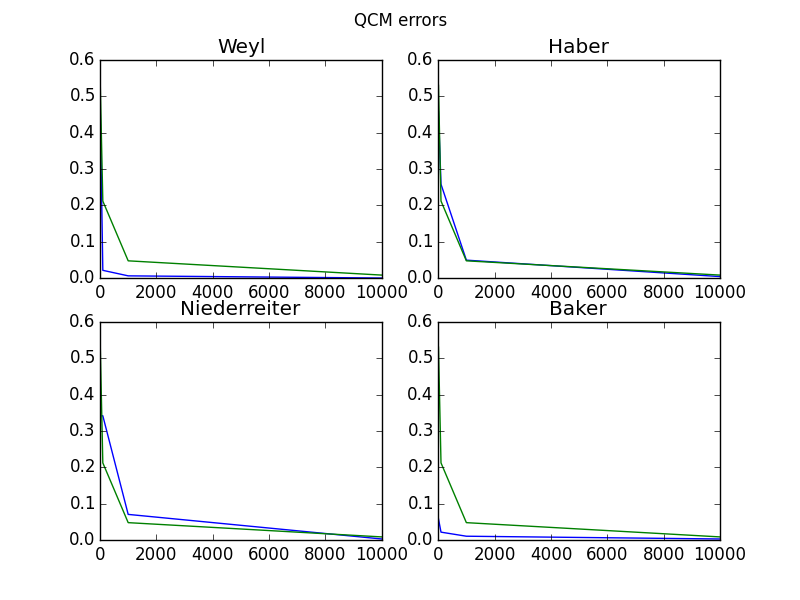
\includegraphics[scale = .75]{QMCerrors}















\end{document}
